\section{Motivation}
\begin{comment}
\subsection{Motivation}
\begin{frame}
	\scriptsize
	\begin{block}{In the earlier work}
		\begin{itemize}
			\item <1-> Focus on a system of partial differential equations which couples a kinetic equation to a macroscopic flow equation. This system model (given by Helzel $\&$ Tzavaras) a sedimentation process in suspension of rigid rod-like particles.
			\item <2-> Study the coupled system on $S^1$
			\item <3-> Construction a lower-dimensional model by using a hierarchy of moment equations
			\item <4-> The moment equations are a hyperbolic system with a source term
			\begin{align*}
				\partial_t Q(x,t) + A\partial_x Q(x,t) = \phi(Q(x,t))
		    \end{align*}
			The update of the source term is equivalent to a spectral method (\cite{doi:10.1137/21M1464592}).
		\end{itemize}
	\end{block}
	\begin{block}{General about the project}
		\begin{itemize}
			\item <5->  Study the coupled system on $S^2$, which is a five dimensional problem (plus time)
			\item <6-> Reduction of the higher-dimensional model by a three-dimensional system of partial differential equations
		\end{itemize}
	\end{block}
	\begin{block}{First step}
		\begin{itemize}
			\item <7-> Derive a spectral Method for the Smoluchowski Equation on $S^2$
			\item <8-> 
		\end{itemize}
	\end{block}
\end{frame}
\end{comment}

\begin{frame}
	\begin{figure}[H]
		\centering
		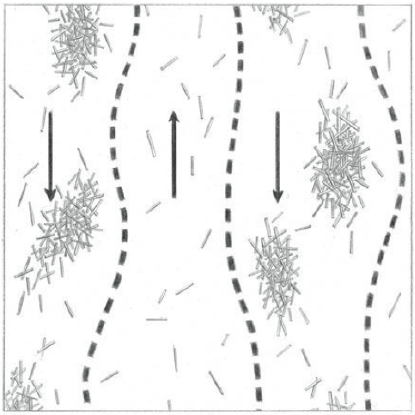
\includegraphics[scale=0.45]{Bilder/Bild_Particles}
		\caption{A suspension of rod-like particles in a dilute solution under the influence of gravity \cite{zbMATH05990161}.}
	\end{figure}
\end{frame}
\begin{frame}{Mathematical Model for the Sedimentation of Rod-Like Particles}
	\scriptsize
	\text{Coupling of a kinetic Smoluchowski equation with Navier-Stokes equation}
	\begin{align*}
		\textcolor{blue}{\partial_t f}+\nabla_{\boldsymbol{x}} \cdot(\boldsymbol{u} f) & +\textcolor{blue}{\nabla_{\boldsymbol{n}} \cdot\left(P_{\boldsymbol{n}^{\perp}} \nabla_{\boldsymbol{x}} \boldsymbol{u} \boldsymbol{n} f\right)}-\nabla_{\boldsymbol{x}} \cdot\left((I+\boldsymbol{n} \otimes \boldsymbol{n}) e_3 f\right) \\
		& =\textcolor{blue}{D_r \Delta_n f}+\gamma \nabla_{\boldsymbol{x}} \cdot(I+\boldsymbol{n} \otimes \boldsymbol{n}) \nabla_{\boldsymbol{x}} f, \notag \\
		\sigma & =\int_{S^{d-1}}(\text{d} \; \boldsymbol{n} \otimes \boldsymbol{n}-I) f d \boldsymbol{n},  \\
		\operatorname{Re}\left(\partial_t \boldsymbol{u}+\left(\boldsymbol{u} \cdot \nabla_{\boldsymbol{x}}\right) \boldsymbol{u}\right) & =\Delta_{\boldsymbol{x}} \boldsymbol{u}-\nabla_{\boldsymbol{x}} p+\delta \gamma \nabla_{\boldsymbol{x}} \cdot \sigma-\delta \int_{S^{d-1}} f d \boldsymbol{n} \, e_3, \\
		\nabla_{\boldsymbol{x}} \cdot \boldsymbol{u} & =0,
	\end{align*}
	where $f = f(t, x, n), x \in \mathbb{R}^3 , n \in  S^2, t \in \mathbb{R}$ is a density distribution function of particle orientation. $D_r, \gamma, \delta$ and $Re$ are non-dimensional parameters.
	
	\begin{beamercolorbox}[sep=1em,wd=\linewidth,right]{}
		\tiny{Helzel $\&$ Tzavaras, 2017}
	\end{beamercolorbox}
\end{frame}

\begin{frame}{A Hierarchy of Moment Equations for a Simplified Model}
	\scriptsize
	Consider simplified flow problem with $\boldsymbol{u} = (0,0, w(x,t))^T$ and $f=f(t,x,\theta)$. Using $\gamma = 0$ the coupled system reads
	\begin{align*}
		\partial_t f(t,x,\theta) +  \textcolor{cyan}{\partial_\theta(w_x \cos^2 \theta f)} - \partial_x (\sin \theta \cos \theta f) &=  \textcolor{cyan}{D_r \partial_{\theta\theta} f} \\
		R e \partial_t w &=\partial_{x x} w+\delta\left(\bar{\rho}-\int_0^{2 \pi} f d \theta\right)
	\end{align*}

	Hierarchy of moment equations:
	\begin{align*}
		\partial_t \rho(x, t) & = \partial_x S_1 \\
		\partial_t C_{\ell}(x, t) & = \frac{1}{4} \partial_x\left(S_{\ell+1}-S_{\ell-1}\right)- \textcolor{cyan}{\frac{\ell}{2} w_x\left(S_{\ell-1}+2 S_{\ell}+S_{\ell+1}\right)}- \textcolor{cyan}{4 \ell^2 D_r C_{\ell}}, \\
		\partial_t S_{\ell}(x, t) & =\frac{1}{4} \partial_x\left(C_{\ell-1}-C_{\ell+1}\right)+  \textcolor{cyan}{\frac{\ell}{2} w_x\left(C_{\ell-1}+2 C_{\ell}+C_{\ell+1}\right)}- \textcolor{cyan}{4 \ell^2 D_r S_{\ell}}, \quad \ell=1,2, \ldots
	\end{align*}

	Compare:
	
	\begin{align*}
		\partial_t f + \textcolor{cyan}{\partial_\theta(w_x \cos^2 \theta f)} = \textcolor{cyan}{D_r \partial_{\theta\theta} f} \quad \text{and} \quad \partial_t Q(x,t) = \textcolor{cyan}{\phi(Q(x,t))}
	\end{align*}
	
	\begin{beamercolorbox}[sep=1em,wd=\linewidth,right]{}
		\tiny{Dahm $\&$ Helzel, 2022}
	\end{beamercolorbox}
\end{frame}

\begin{frame}{Goal}
	\scriptsize
	\begin{block}{General about the project}
		\begin{itemize}
			\item <1->  Study the coupled system on $S^2$, which is a five dimensional problem (plus time)
			\item <2->  Transform this high dimensional system into a lower dimensional system of moment equations
		\end{itemize}
	\end{block}
	\begin{block}{First step}
		\begin{itemize}
			\item <3-> Derive a Spectral Method for the Smoluchowski Equation on $S^2$
		\end{itemize}
	\end{block}
	
\end{frame}

